%%%% CAPÍTULO 1 - INTRODUÇÃO
%%
%% Deve apresentar uma visão global da pesquisa, incluindo: breve histórico, importância e justificativa da escolha do tema,
%% delimitações do assunto, formulação de hipóteses e objetivos da pesquisa e estrutura do trabalho.

%% Título e rótulo de capítulo (rótulos não devem conter caracteres especiais, acentuados ou cedilha)
\chapter{Introdução}\label{cap:introducao}

Um texto curto apresentando o capítulo.

\caixa{Atenção}{Para utilizar esse template é obrigatória a leitura do conteúdo do arquivo \texttt{readme.md}, que está neste projeto!}
\section{Considerações iniciais}\label{sec:consideracoesIniciais}

As considerações iniciais compõem um texto curto e geral apresentando uma visão geral e sucinta do assunto principal relacionado ao trabalho e a inserção do objeto de pesquisa nesse assunto \cite{Moore:2000:CMC:333067.333074}.

\noindent Exemplos de citação:

Segundo \citeonline{Coulouris2013}.

Segundo \citeonline[p. 40]{Coulouris2013}.

Citação no final do Parágrafo~\cite{Coulouris2013}. 

Citação no final do Parágrafo com número de página~\cite[p. 40]{Coulouris2013}.

%(Modelo de referência: pessoa jurídica)
Citação no final do Parágrafo~\cite{NBR6023:2018}

%(Modelo de referência: pessoa jurídica)
Citação no final do Parágrafo~\cite{NBR6027:2012}

%(Modelo de referência: pessoa jurídica)
Citação no final do Parágrafo~\cite{NBR6028:2021}

Segundo a \citeonline{NBR14724:2011}.

Citação no final do Parágrafo~\cite{NBR10520:2002}

Citação no final do Parágrafo~\cite{NBR14724:2011}.

% (Modelo de referência de trabalho acadêmico).
Citação no final do Parágrafo~\cite{Andrade2005}

% (Modelo de referência: capítulo de livro).
Citação no final do Parágrafo~\cite{Borges2014}

% (Modelo de referência: leis, decretos, portarias, etc.)
Citação no final do Parágrafo~\cite{BRASIL:1998}

% (Modelo de referência: livro com subtítulo). Nome com sufixo "Von" - Configuração no bib
Citação no final do Parágrafo~\cite[p. 66]{KROGH:2001}

Citação no final do Parágrafo~\cite{Faina2001}

% (Modelo de referência: livro com subtítulo).
Citação no final do Parágrafo~\cite{Davenport2012}

% (Modelo de referência: artigo de periódico).
Citação no final do Parágrafo~\cite{Monteiro2009}

%(Modelo de referência: artigo de periódico). Nome familiar "Junior"
Citação no final do Parágrafo~\cite{Sanches2024}

% (Modelo de referência: trabalho publicado em evento).
Citação no final do Parágrafo~\cite{Renaux2001}

Em relação ao assunto, o apresentado nesta seção pode estar relacionado a trabalhos de outros autores ou ao assunto que fornece a fundamentação (motivação) para o trabalho a ser desenvolvido. Se o assunto está relacionado a trabalhos de outros autores, a contribuição do trabalho é definida em relação ao que já foi pesquisado nesse assunto. Se o assunto será utilizado para embasamento do que será proposto, explicitar como o trabalho se insere nesse assunto. A contribuição pode, ainda, estar relacionada a uma necessidade de mercado ou a uma oportunidade decorrente de algum problema real para o qual se pretender propor uma solução. Nesse caso, o assunto fornece um contexto teórico de suporte para o problema e/ou a solução.

O importante nesta seção é deixar claro do que se trata o trabalho (assunto ou tema), identificar o objeto de pesquisa, como será encaminhada a solução (procedimento metodológico, tecnologias, ferramentas utilizadas) e o que se pretende ao final do trabalho, sem explicitar a solução e os resultados.

\caixa{Atenção}{As seções a seguir são sugestões, converse com o seu orientador para ver quais seções devem ter em seu trabalho!}

\begin{photograph}[!htb]%% Ambiente figure
    %\captionsetup{width=0.55\textwidth}%% Largura da legenda
    \caption{Exemplo de fotografia}%% Legenda
    \label{fig:exemplo1}%% Rótulo
    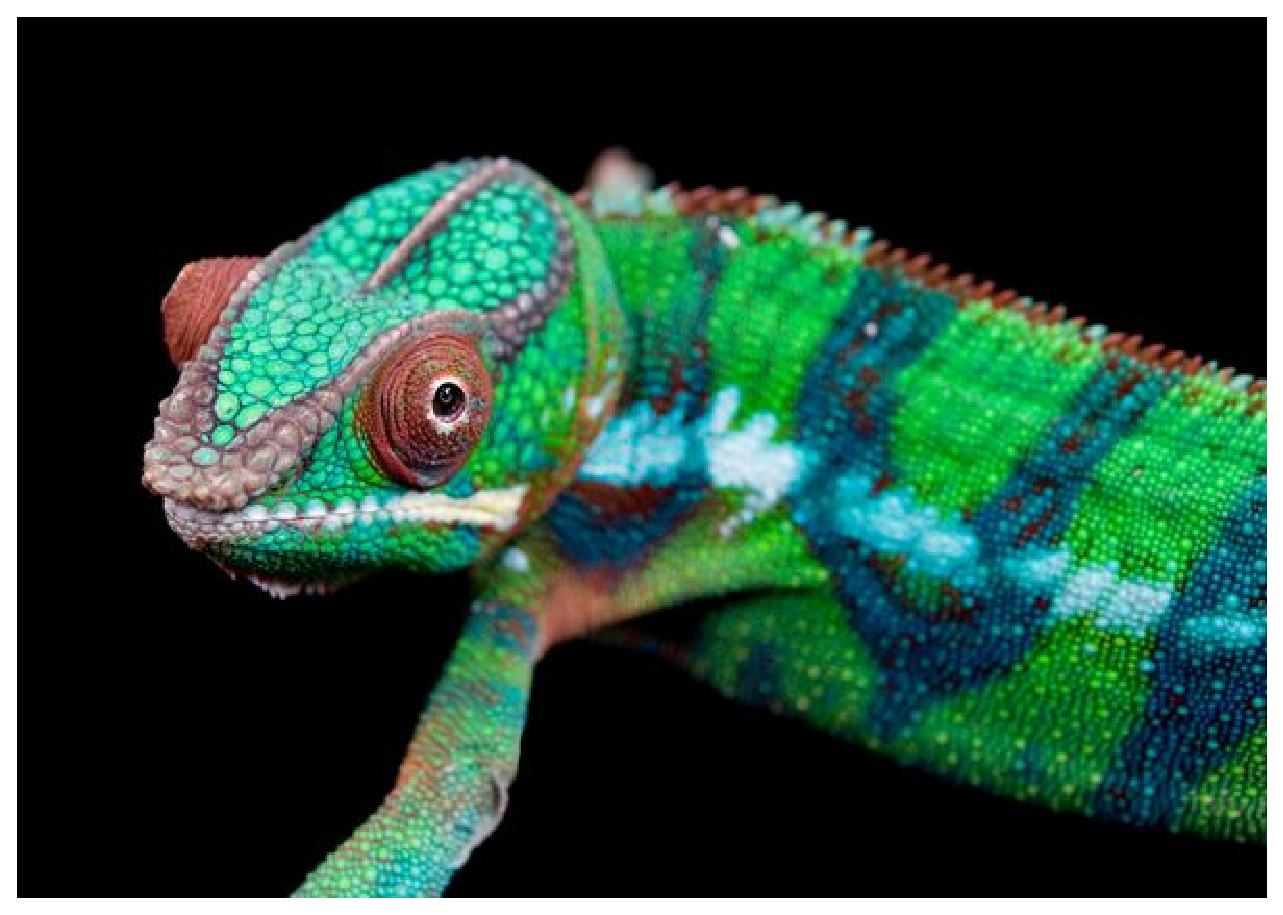
\includegraphics[scale=0.4]{foto1}%% Dimensões e localização
    \fonte{Autoria Própria}%% Fonte
    \addcontentsline{loge}{photograph}{\protect\numberline{\thephotograph}Exemplo de fotografia.} % Adiciona à lista de ilustrações
\end{photograph}


\section{Objetivos}\label{sec:objetivos}

Um texto curto\footnote{Teste de nota de rodapé 1.} apresentando a seção.



\section{Objetivos específicos (opcional)}\label{subsec:objetivosEspecificos}

Os objetivos específicos são opcionais, ou seja, somente devem ser apresentados se caracterizarem resultados parciais gerados a partir do objetivo geral, os quais sejam considerados úteis para a comunidade acadêmica, para a sociedade ou para o ambiente profissional. Uma observação importante é que os resultados sejam passíveis de comprovação, ou seja, se o objetivo for: “Oferecer agilidade e confiabilidade aos processos gerenciais da empresa”, significa que o trabalho deverá realizar testes com relação a esses atributos, cujos resultados deverão ser apresentados nas discussões do trabalho.

\begin{graph}[!htb]%% Ambiente figure
    %\captionsetup{width=0.55\textwidth}%% Largura da legenda
    \caption{Exemplo de gráfico}%% Legenda
    \label{graph1}%% Rótulo
    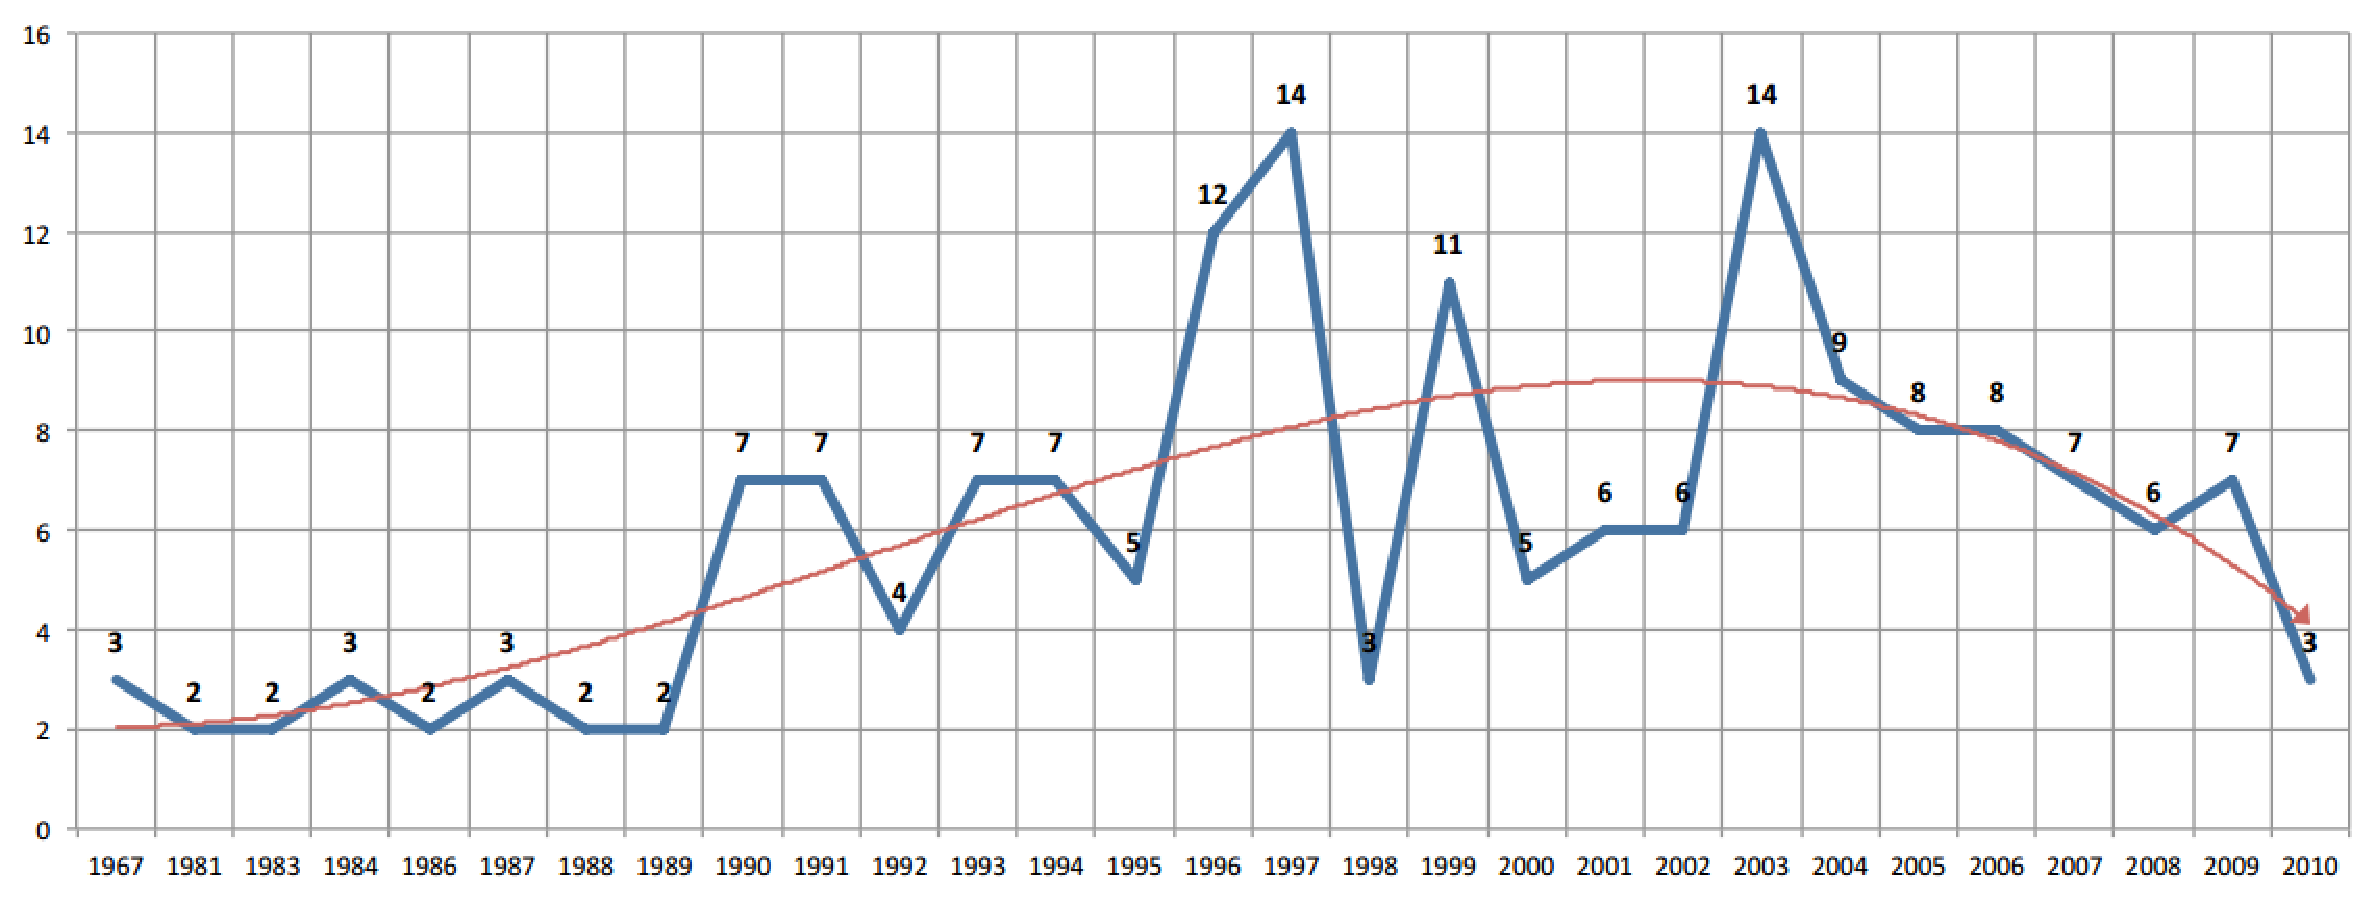
\includegraphics[scale=0.4]{grafico2}%% Dimensões e localização
    \fonte{Adaptado de \citeonline[p.~4]{UTFPR2008}}%% Fonte
    \addcontentsline{loge}{graph}{\protect\numberline{\thegraph}Exemplo de gráfico.}
\end{graph}


Destaca-se que os objetivos específicos não incluem as etapas do processo de desenvolvimento de software (realizar a modelagem, a análise, o projeto...) ou outras atividades necessárias para alcançar o objetivo geral, como, estudar as tecnologias necessárias para modelagem e implementação do sistema. Dentre as exceções estão a realização de estudos, procedimentos, métodos e técnicas considerados inéditos e de relevância para outros trabalhos a serem realizados na mesma área. Contudo, o resultado deste estudo deve ser documentado de forma que seja conhecimento disponibilizado para quem lê o trabalho.

\subsection{Seção ternária (sublinhado)}

xxxxxxxx mkmdasda

asdadas

 
\subsubsection{Seção quaternária (sublinhado)}

xxxxxxxxx

dasda

\subsubsubsection{Seção quinária (itálico)}

\section{Justificativa}\label{sec:justificativa}

Justificar o objeto de pesquisa (o que será feito) e a forma de resolução do problema (como fazer). A forma de resolução pode estar centrada no método, nas tecnologias, no uso de conceitos (fundamentação teórica).

A Justificativa explicita porque desenvolver o referido trabalho, como o mesmo se insere no contexto de pesquisa, de produção científica. Pode incluir o porquê utilizar as tecnologias e ferramentas indicadas, a contribuição em termos de inovação ou mesmo de aprendizado.

O trabalho não precisa ser justificado em decorrência de ser inovador ou por ter gerado uma significativa contribuição ao conhecimento na área em que o mesmo se insere. Pode referir-se simplesmente à aplicabilidade de conhecimentos adquiridos durante o curso. Sendo assim, a justificativa não deve ser elaborada considerando um mercado a ser atingido e sim com relação ao uso de tecnologias aprendidas e/ou estudadas, o conhecimento e aprendizado do aluno e a aplicabilidade do trabalho desenvolvido.

\section{Estrutura do trabalho}\label{sec:estruturaTrabalho}

A estrutura do trabalho contém uma relação dos capítulos e uma descrição sucinta do que cada um deles contém. Esta seção fornece uma visão geral do trabalho no sentido da sua estrutura em capítulos\footnote{Teste de nota de rodapé 2.}.

\caixa{Atenção}{O OverLeaf está demorando muito para compilar o modelo com o Capítulo de Exemplos, que explica como usar o LaTeX. Assim, esse capítulo foi removido (está comentado para não compilar), mas há um arquivo chamado \texttt{exemploPDF.pdf}, na raiz do projeto, que contém esse capítulo de exemplos!}


